\documentclass[8pt]{article}
\usepackage{graphicx}
	\setkeys{Gin}{width=0.4\textwidth}
\usepackage[a4paper]{geometry}
\usepackage{listings}
\twocolumn
\begin{document}
	\author{Jonathan Cancio \\ Oliver Atienza \\ Justin Balderas \\ 
	Reyster Fresco \\ Yna Ojeda \\ Ethan Tan \\ Marc Teves \\ Troy Valdez}
	\title{CS 131 MP2}
	\maketitle
	\section{Abstract}
	% Make sure to always have one sentence per line.
	Predicting the future price of shares in a particular company will allow stock traders to make more profitable trades.
	The group tried to predict the closing price of seven different companies on 24 May 2018. 
	The group performed a linear regression on their closing price and trading volume over varying timespans.
	The prediction error was found to be (to be continued...)
	\section{Introduction}

	\section{Methodology}

	\begin{figure}[h]
		\centering
		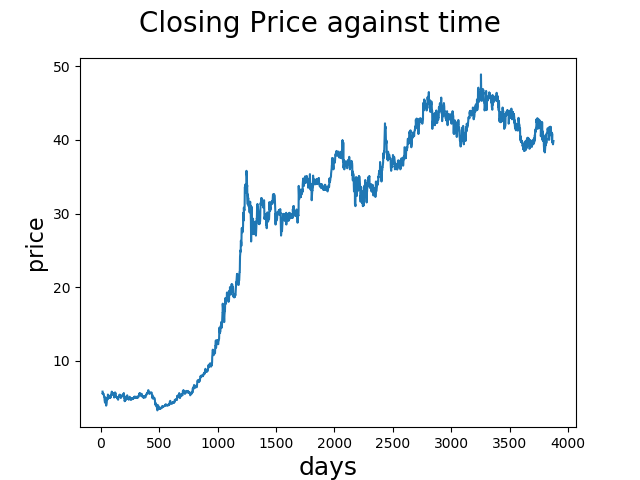
\includegraphics{ap_closing_price.png}
		\caption{Closing prices}
		\label{fig:close_price_graph}
	\end{figure}

	Take a look at Figure~\ref{fig:close_price_graph}. On the x-axis is
	\texttt{days} and the y-axis is \textbf{price}
	\subsection{Preprocessing}
	In this section we take a look at the data processing required to make the
	data workable.
		\subsubsection{Removing irrelevant companies}
		Go through each entry one by one and delete it if it's not one of the tracked companies.

	\section{Results}
	\section{Discussion}
	\section{Conclusion}
	\begin{thebibliography}{9}
		\bibitem{heath}
			Heath M.,

			\textit{Scientific Computing - An Introductory Survey}
	\end{thebibliography}
\end{document}
